\def\theTopic{Inference on Proportions }
\def\dayNum{8}

\begin{center}
{\bf {\large MIT -- the Male Idiot Theory}}
\end{center}

The usually  serious {\em British Medical Journal} enjoys a bit
of fun in each Christmas issue.  In December 2014 they
published a study of the MIT -- ``Males are Idiots Theory'' based on
data collected from the Darwin Awards.

``Winners of the Darwin Award must die in such an idiotic
manner that `their action ensures the long-term survival of the
species, by selectively allowing one less idiot to survive.'$^{20}$ The
Darwin Awards Committee attempts to make a clear distinction
between idiotic deaths and accidental deaths. For instance,
Darwin Awards are unlikely to be awarded to individuals who
shoot themselves in the head while demonstrating that a gun is
unloaded. This occurs too often and is classed as an accident.
In contrast, candidates shooting themselves in the head to
demonstrate that a gun is loaded may be eligible for a Darwin
Award--such as the man who shot himself in the head with a
`spy pen' weapon to show his friend that it was real.$^{18}$
To qualify, nominees must improve the gene pool by eliminating
themselves from the human race using astonishingly stupid
methods. Northcutt cites a number of worthy candidates.$^{12-21}$
These include the thief attempting to purloin a steel hawser from
a lift shaft, who unbolted the hawser while standing in the lift,
which then plummeted to the ground, killing its occupant; the
man stealing a ride home by hitching a shopping trolley to the
back of a train, only to be dragged two miles to his death before
the train was able to stop; and the terrorist who posted a letter
bomb with insufficient postage stamps and who, on its return,
unthinkingly opened his own letter.''\footnote{Lendrem, B. A. D.,
  Lendrem, D. W., Gray, A., \& Isaacs, J. D. (2014). The Darwin
  Awards: sex differences in idiotic behaviour. BMJ, 349, g7094.} 

The authors examined 20 years of data on the awards, removing awards
given to couples ``usually in compromising positions'' so that each
remaining winner was either male or female. Of the 318 remaining
awards, 282 were given to males and 36 were awarded to females.

They ask the question: ``If we look only at  people who do really
stupid things, what is the gender breakdown?''  or ``Are idiots more
than half male?''

\begin{enumerate}
   \item  What population is  represented by these winners of the
     Darwin Awards?
\begin{students}
    \vspace{1.6cm}    
\end{students}
\begin{key}
  {\it One could answer that winners of the award are their own small
    population, and we have a census of all Darwin Award
    winners. However, there are other idiots who have not yet won this
    competition, but seem to be working toward proving themselves. I
    would say that the sample observed represents a population of people who
    take risks which should be avoided.} 
\end{key}
   \item  What is the parameter of interest?
\begin{students}
    \vspace{1cm}    
\end{students}
\begin{key} 
  {\it $p$ = the proportion of all idiots who are male.}
\end{key}
  \item \label{MIT.phat} What statistic do we obtain from the sample?
    Give proper notation, the statistic's value, and explain it in words.
\begin{students}
    \vspace*{2cm}    \\
\end{students}
\begin{key} 
   { $\widehat{p} = \frac{282}{318} = 0.887$ \it is the
    proportion of the sample which is male.}
\end{key}
\item Looking at the research question, ``Is the group of idiots in the world
  more than half male?'',   we set
  up the null hypothesis to assume ``just half'' and the alternative to be
  ``more than half'' male.
    \begin{enumerate}
    \item State null and alternative hypotheses in symbols and
      words.\\
      $H_0:$ 
\begin{students}
    \vspace{1.5cm}    \\
\end{students}
\begin{key} 
{\it $p = .5$.  Half of all idiots are male.}
\end{key}
$H_a:$
\begin{students}
    \vspace{1cm}    \\
\end{students}
\begin{key} 
{\it $p > .5$.  More than half of all idiots are male.}
\end{key}
    \item How would you mark cards and randomly draw from them to
      obtain one simulated proportion drawn from the distribution when
      $H_0$ is true?
\begin{students}
    \vspace{3cm}    
\end{students}
\begin{key} 
  {\it Take an even number of cards (could be 318, but a
    smaller number will also work). Mark half of them male, half
    female. Shuffle and draw one. Record the gender. Return the card
    to the deck, repeat 317 more times and divide the total number of
    males by 318 to get one sample proportion.}
\end{key}
    \item Input the data under ``One Categ'' in 
      \url{http://shiny.math.montana.edu/jimrc/IntroStatShinyApps/} and use
      the  ``Test'' page to obtain
      the distribution of 1000 or more sample proportions under $H_0$.
      Sketch the picture you get here.
\begin{students}
    \vspace{5cm}    
\end{students}
\begin{key}
\ \  \\ 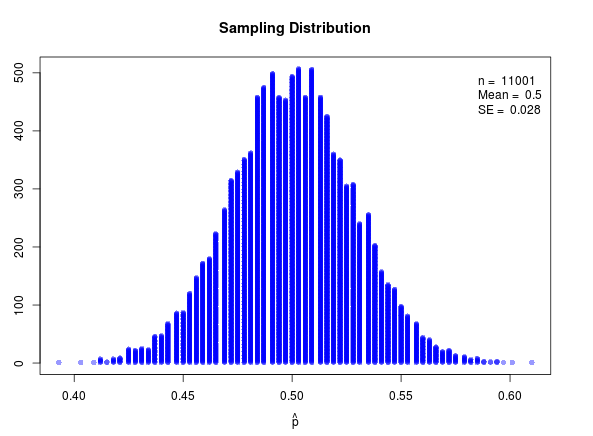
\includegraphics[width=.3\linewidth]{plots/MIT-null.png}
\end{key}
  \item How unusual is the sample statistic from \ref{MIT.phat}
    relative to the distribution you created?  Explain in words where
    it falls relative to the plotted points.
\begin{students}
    \vspace{3cm}    
\end{students}

\begin{key}
{\it It's much bigger than any of the points I generated. The largest
  one I got was 0.585 or 186 males out of 318.}
\end{key} 
\item  How strong is the evidence against the null hypothesis?  What
  do you think about the idea that idiots are half male?
\begin{students}
    \vspace{2cm}    
\end{students}

\begin{key}
  {\it Extremely strong evidence, the p-value is less than 1 in
    1000. The null hypothesis of only half males is not 
    supported by these data. I conclude that there are more male idiots
  than female idiots.  } 
\end{key}


\end{enumerate}

\item Instead of considering a test of the true population proportion, we
  will switch gears and now estimate it.
  \begin{enumerate}
    \item What is our ``point'' estimate of the
      true proportion of idiots who are male (the sample statistic)?
\begin{students}
    \vspace{.4cm}    
\end{students}

\begin{key}
$\widehat{p} = 0.887$
\end{key}
    \item In order to generate simulated data,
      \begin{enumerate}
        \item How many individual ``idiots'' do we generate for one
          resample?
\begin{students}
    \vspace{.8cm}    
\end{students}

\begin{key} 
$318$
\end{key}
       \item Explain how you would mark 318 cards and use them to
         simulate the gender of one individual, and then another.
\begin{students}
    \vspace{2.5cm}    
\end{students}

\begin{key} 
  {\it Mark 26 ``Female'' and 282 ``Male''.  Shuffle them and draw one
  at random.  Replace the card, remix, and draw again for the second
  person.} 
\end{key}
       \item What probability of being male is used?
\begin{students}
    \vspace{.5cm}    
\end{students}

\begin{key} 
  {$0.887$}
\end{key}
       \item After resampling 318 individuals, what number do you compute?
\begin{students}
    \vspace{1.2cm}    
\end{students}

\begin{key} 
  {\it  The proportion of the 318 new draws which are male.}
\end{key}
     \end{enumerate}
     \item Use the  web applet to create  1000 or more
       resamples from the original data. Plug in the numbers from the data.
       \begin{enumerate}
         \item Where is this distribution centered?
\begin{students}
    \vspace{.7cm}    
\end{students}

\begin{key} 
  {\it  0.887}
\end{key}
         \item What is the spread of the distribution of resampled proportions?
\begin{students}
    \vspace{.7cm}    
\end{students}

\begin{key} 
  {\it SE =  0.018}
\end{key}
         \end{enumerate}
     \item Find a 95\% confidence interval for the true proportion of
       idiots who are male.
\begin{students}
    \vspace{1.2cm}    
\end{students}

\begin{key} 
  $  (0.852, 0.925)$
\end{key}
     \item \label{longRun}Explain what the word ``confidence'' means for this
       confidence interval.
\begin{students}
    \vspace{3cm}    
\end{students}

\begin{key} 
  {\it Our confidence is in the process, not in just one interval. If
    we repeat the process (gather a new random sample) over and over,
    95\% of the intervals we create will include the true parameter of
  interest.}
\end{key}

  \end{enumerate}
\item Compare results from the hypothesis test and the interval
  estimate.  If the null hypothesis is true, what value should be
  included in the 95\% CI?  Explain. Do the two methods agree to some
  extent? 
\begin{students}
    \vspace{4.2cm}    
\end{students}

\begin{key} 
  {\it  If $H_0$ is true, then the interval should contain 0.50.  It
    does not, so the two inferences agree that one--half is not
    consistent with the data.} 
\end{key}
\end{enumerate}


\begin{center}
  {\bf Take Home Message:}
\end{center}
\begin{itemize}
  \item You just did two inferences on the same parameter.  First, we
    tested the null hypothesis that half the world's idiots are
    male.\\
      You should have reported very strong evidence against that null
      hypothesis (less than 1/1000). We can feel quite confident that
      the true proportion 
      of males in this exclusive group is more than one half.

  \item Secondly, we computed a 95\% confidence interval for the true
    proportion of idiots who are male and you interpreted the
    interval.  In \ref{longRun} you should have explained the
    long--run coverage property of the method.
  \item   There is a correspondence
    between testing and estimating.  The values inside the interval
    you found are consistent with the data, or {\bf plausible}.  Because
    0.50 is not in the interval, it is not a plausible value for this
    parameter. 
 \item 
  Use the remaining space for any questions or your own summary of the
  lesson. 

\end{itemize}

%% Not yet using `reject the null' terminology.
